%! Author = crist
%! Date = 09/05/2026
\spacing{1.3}


\section{Masa Atómica Relativa}

Si la masa de un átomo se expresa en g o en kg resulta un número muy pequeño (\( \approx \qty{e-27}{\kg} \)), incómodo de manejar, por lo que es más conveniente utilizar una escala relativa de masas atómicas comparando las masas de los átomos con la masa de un átomo de referencia o patrón. Inicialmente se tomó el H, después el O y actualmente se toma el isótopo más abundante en la Naturaleza, el Carbono–12, al que se le asigna una masa atómica 12.

De esta forma, la masa atómica relativa de un elemento es un número sin dimensiones; por tanto, que la masa atómica de un elemento sea 40, significa que la masa de uno de sus átomos es 40 veces mayor que la doceava parte de la masa de un átomo de Carbono-12.
Aunque masa y peso son magnitudes distintas, la masa atómica relativa y el peso atómico relativo de un elemento coinciden.

También se utiliza una unidad de masa: La unidad de masa atómica (u.m.a., u.a.m. o u), que se define como la doceava parte de la masa de un átomo de C-12.
La masa atómica del C-12 es 12 u.m.a. y es el único átomo que tiene una masa entera, los demás átomos tiene una masa atómica fraccionaria debido al defecto másico.

\begin{figure}[H]
    \centering
    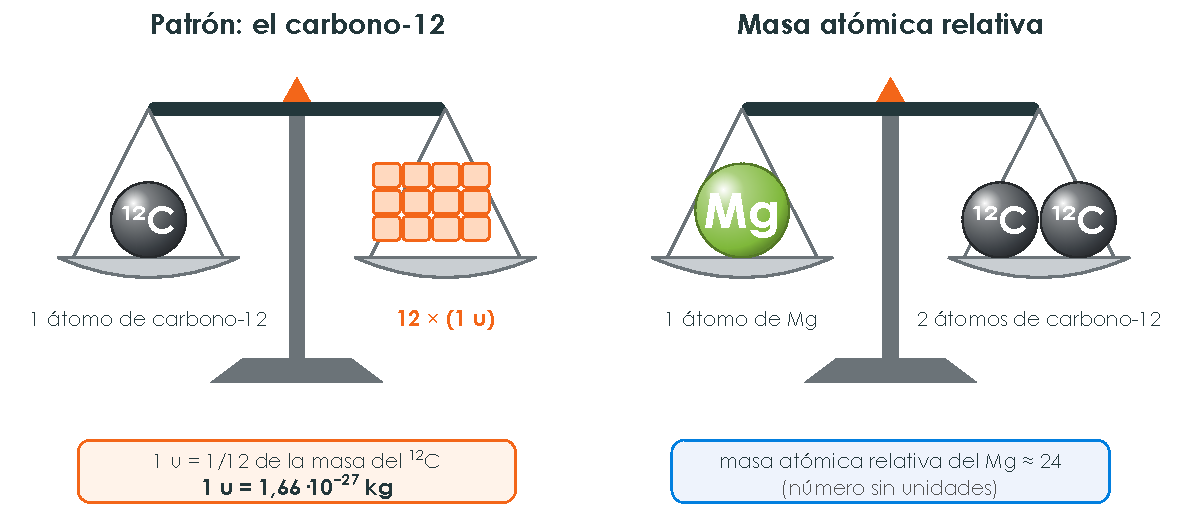
\includegraphics[width=0.75\linewidth]{FigurasSVG/UD0_Conocimientos_Basicos/pdf/UD0_01_unidad_masa_atomica.pdf}
    \caption{Unidad de masa atómica y masa atómica relativa}
    \label{fig:unidad-masa-atomica}
\end{figure}

\textbf{Masa atómica (promedio) de un elemento:} debido a la existencia de isótopos, se toma como masa atómica de un elemento a la masa promediada de sus isótopos.
\begin{centeredequation}
    M_{at}\ = \dfrac{\sum_{i=1}^{n} (\text{Abundancia relativa (en \%)} \times \text{masa atómica del isótopo})}{100}
\end{centeredequation}

\textbf{Masa molecular:} Se obtiene sumando la masa de los átomos que forman la molécula.

En los elementos que forman moléculas, no se debe confundir la masa atómica con la molecular.

En los compuestos iónicos no hay moléculas, sino iones, por lo cual, algunos autores utilizan el término masa fórmula en vez de masa molecular, que se define como la masa de una fórmula de sólido iónico, y se calcula igual que la masa molecular.

\textbf{Mol:} cantidad de sustancia que contiene tantas partículas (átomos, moléculas, iones) como átomos hay en 12 gramos de Carbono-12.
Este número se llama \textbf{Número de Avogadro}  \( N_A = \num{6.022e23} \).

\textbf{ Mol de átomos de un elemento}, es la cantidad de dicho elemento que contiene el \( N_A \) de átomos.
\textbf{Mol de moléculas de un elemento o compuesto}, es la cantidad de dicho elemento o compuesto que contiene el \( N_A \) de moléculas.

\textbf{Masa molar:} es la masa de un mol de una sustancia.
\begin{itemize}
    \item Si es de 1 mol de átomos también se llama átomo-gramo, es la masa del NA de átomos de dicho elemento, y es igual a la masa atómica expresada en gramos.
    \item Si es de 1 mol de moléculas también se llama molécula-gramo, es la masa del NA de moléculas de dicho elemento o compuesto, y es igual a la masa molecular expresada en gramos.
\end{itemize}


\begin{itemize}
    \item M\textsubscript{atómica} H = \qty{1}{\uma} \( \Rightarrow \) masa de 1 mol de átomos (1 átomo-g) de H = \qty{1}{\g} , y contiene \num{6.022e23} átomos de H.
    \item Mmolec. \ch{H2} = 2 u. masa de 1 mol de moléculas(1 molécula-g) de H2 = 2 g , y contiene el NA de moléculas de H2.
    \item Mmolec. \ch{H2O} = 18 u. masa de 1 mol de moléculas (1 molécula-g) de agua = 18 g , y contiene el \( N_A \) de moléculas de \ch{H2O}.
    \item Para hallar el número de moles de átomos o moles de moléculas:
    \begin{centeredequation}
        n = \dfrac{m(g)}{\text{M}_{\text{atómica}}\;\left( \unit{\g\per\mol}\right)}
    \end{centeredequation}
    También se puede hacer utilizando factores de conversión (se recomienda)
    Si partimos de \qty{10}{\g} de \ch{H20} el cálculo de los moles utilizando factores de conversión y sabiendo que la masa molar del \ch{H2O} es \qty{18}{\g\per\mol}:
    \begin{centeredequation}
        18 \cancelred{\unit{\g}} \cdot \dfrac{1\ \unit{\mol}}{18 \cancelred{\unit{\g}}} = \qty{1}{\mol}
    \end{centeredequation}
\end{itemize}


\begin{figure}[H]
    \centering
    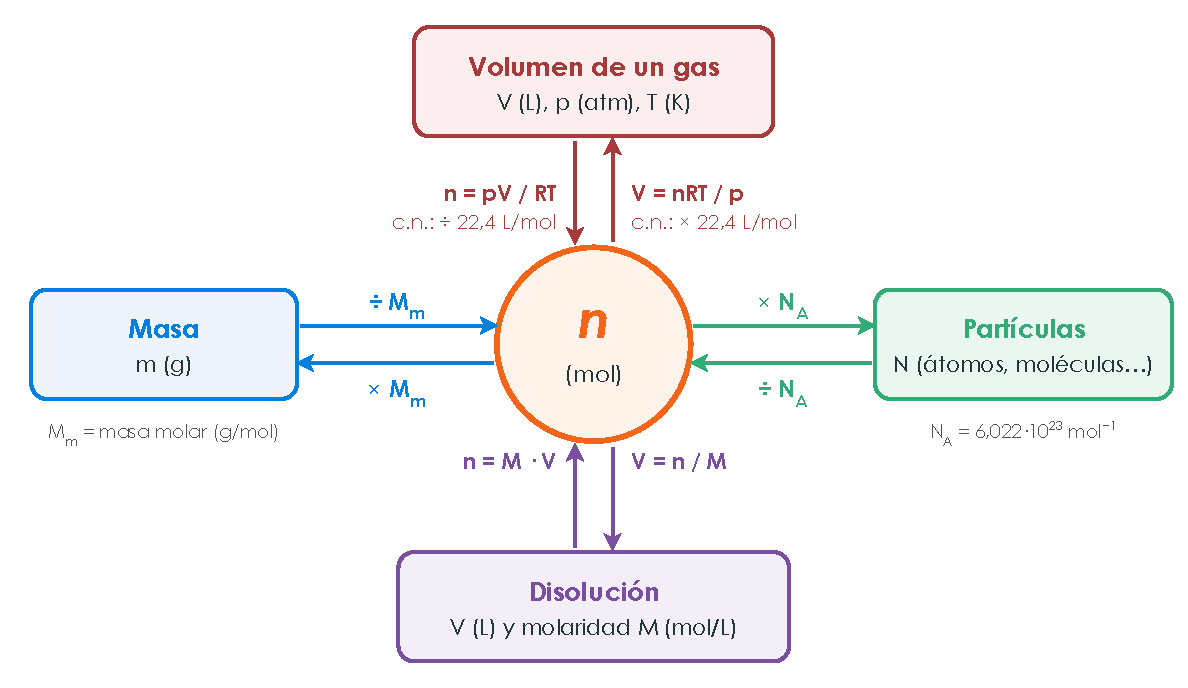
\includegraphics[width=0.8\linewidth]{FigurasSVG/UD0_Conocimientos_Basicos/pdf/UD0_02_mol_magnitud_central.pdf}
    \caption{El mol como magnitud central de los cálculos químicos}
    \label{fig:mol-magnitud-central}
\end{figure}

\section{Disoluciones}
\begin{definition}[Disolución]
    es una mezcla homogénea de dos o más sustancias puras y de composición variable, es decir, su composición y propiedades son las mismas en todos los puntos y además la composición se puede modificar.
\end{definition}

En una disolución tiene lugar la dispersión, la difusión, de las partículas de una sustancia llamada soluto entre las partículas de otra sustancia llamada disolvente.
Para distinguir el soluto del disolvente, hay que tener presente que el disolvente siempre tiene el mismo estado físico que la disolución y si ambos componentes tienen el mismo estado físico que la disolución, se toma como disolvente el que esté en mayor cantidad. Dependiendo del estado físico de los componentes hay 9 tipos de disoluciones, las más importantes son las disoluciones sólido-líquido y dentro de estas, las disoluciones acuosas, en las que se toma el agua como disolvente, aunque esté en menor cantidad.

\begin{figure}[H]
    \centering
    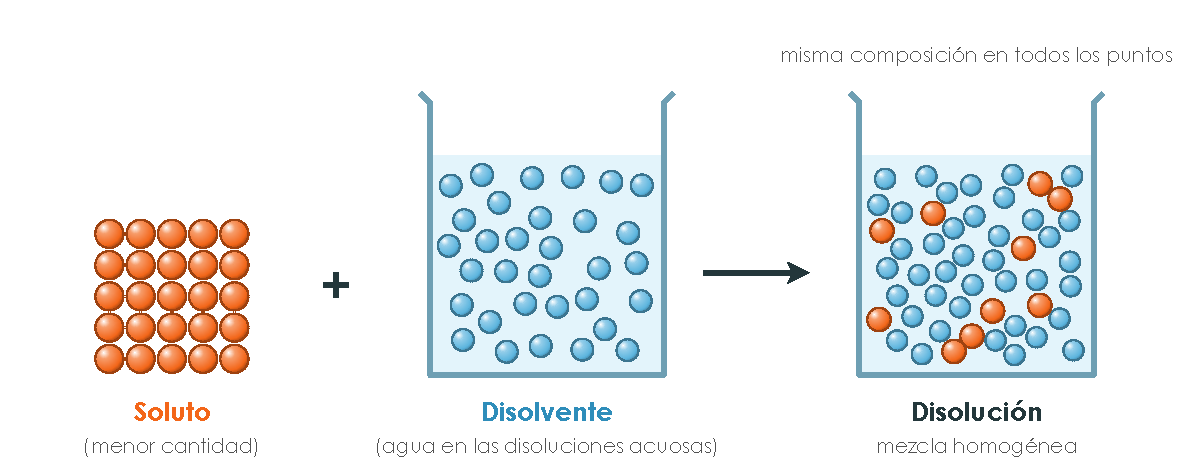
\includegraphics[width=0.8\linewidth]{FigurasSVG/UD0_Conocimientos_Basicos/pdf/UD0_03_disolucion_soluto_disolvente.pdf}
    \caption{El soluto se dispersa entre las partículas del disolvente}
    \label{fig:soluto-disolvente}
\end{figure}

\subsection{Concentración de una disolución}

\begin{definition}[Concentración]
    La \textbf{concentración} de una disolución indica la composición de la misma, es decir, la proporción entre el soluto y el disolvente
\end{definition}
, y se puede expresar de varias formas:
\begin{itemize}
    \item \textbf{\% en masa}: indica la masa de soluto que hay disueltos en 100 unidades de masa de disolución.
    \begin{centeredequation}
        \text{\% en masa} = \dfrac{\text{masa de soluto}}{\text{masa de disolución}} \times 100
    \end{centeredequation}
    \item \textbf{\% en volumen}: indica el volumen de soluto que hay disueltos en 100 unidades de volumen de disolución.
    \begin{centeredequation}
        \text{\% en volumen} = \dfrac{\text{volumen de soluto}}{\text{volumen de disolución}} \times 100
    \end{centeredequation}
    \item \textbf{g/L}: indica los gramos de soluto que hay disueltos en \qty{1}{\litre} de disolución.
    \begin{centeredequation}
        \text{g/L} = \dfrac{\text{m(g) de soluto}}{\text{V (L) de disolución}}
    \end{centeredequation}
    \begin{remark}
        Es importante no confundirlo con la densidad, en este caso el volumen es de la \textbf{disolución} mientras que la densidad nos dice la masa que hay por unidad de volumen de ese compuesto.
    \end{remark}
    \item \textbf{Molaridad (M)}: indica el número de moles disueltos en \qty{1}{\litre} de disolución.
    \begin{centeredequation}
        M = \dfrac{\text{n de soluto}}{\text{V (L) de disolución}}
    \end{centeredequation}
    Los moles (n) los podemos calcular:
    \begin{centeredequation}
        n = \dfrac{\text{m (g) de soluto}}{\text{M}_{\text{molar}} \left(\unit{g\per\mol} \right)}
    \end{centeredequation}
    \item \textbf{Normalidad (N)}: indica los equivalentes-gramo de soluto que hay disueltos en \qty{1}{\litre} de disolución.
    \begin{centeredequation}
        N = \dfrac{\text{nº de eq-g}}{\text{V (L) de disolución}}
    \end{centeredequation}
    El equivalente-gramo, representado como \textbf{eq-g} es una unidad de medida química que representa la cantidad de una sustancia que reacciona con, o sustituye a, una cantidad estándar de otra sustancia química específica.
    \begin{centeredequation}
        \text{eq-g} = \dfrac{\text{m (g) de soluto}}{\text{P}_\text{eq}}
    \end{centeredequation}

    A diferencia del mol, que es una medida de sustancia basada puramente en el número de partículas, el equivalente-gramo depende de la \textbf{reactividad} de la sustancia y del tipo de reacción que tengamos. Siendo P\textsubscript{eq}:
    \begin{centeredequation}
        \text{P}_{\textsubscript{eq}} = \dfrac{\text{Masa molar}}{\text{valencia}}
    \end{centeredequation}
    La \textbf{valencia} es el número de \ch{H+} o \ch{OH-} transferidos en una reacción ácido-base o el número de electrones que ha perdido o ganado en una reacción redox.

    Podemos relacionar fácilmente la normalidad con la molaridad según la ecuación:
    \begin{centeredequation}
        N = M \cdot \text{valencia}
    \end{centeredequation}
    \item \textbf{Molalidad (m)}: indica los moles de soluto disueltos en \qty{1}{\kg} de disolvente.
    \begin{centeredequation}
        m = \dfrac{\text{n de soluto}}{\text{Kg de disolvente}}
    \end{centeredequation}
    \item \textbf{Fracción molar del soluto (\( \chi_{s} \))}: indica los moles de soluto disueltos en \qty{1}{\mol} de disolución y se representa con el símbolo \( \chi_s \). Su valor siempre está entre 0 y 1.
    \begin{centeredequation}
        \chi_{s} = \dfrac{\text{moles de soluto}}{\text{moles de disolución}} = \dfrac{\text{moles de soluto}}{\text{moles de soluto} + \text{moles de disolvente}}
    \end{centeredequation}
    \item \textbf{Fracción molar del disolvente}: indica los moles de disolvente que tenemos en \qty{1}{\mol} de disolución y se representa con \( \chi_d \). Su valor también está entre 0 y 1.
    \begin{centeredequation}
        \chi_{d} = \dfrac{\text{moles de disolvente}}{\text{moles de disolución}} = \dfrac{\text{moles de disolvente}}{\text{moles de soluto} + \text{moles de disolvente}}
    \end{centeredequation}
    Se cumple también que:
    \begin{centeredequation}
        \chi_s + \chi_d = 1
    \end{centeredequation}
\end{itemize}


\section{Leyes de los gases}

\subsection{Ley de los gases ideales}

\begin{definition}[Gas ideal]
    es una sustancia simple compresible y pura de naturaleza especial y se considera un modelo \textbf{teórico} o \textbf{hipotético} en el que sus partículas se desplazan aleatoriamente y no \textbf{interactúan entre sí} y por tanto no existen fuerzas de atracción o repulsión.
\end{definition}

Las leyes de Boyle-Mariotte, Charles y Gay-Lussac se pueden combinar en una ecuación general denominada ecuación general de los gases ideales:

\begin{centeredequation}
    p\cdot V = n \cdot R \cdot T
\end{centeredequation}

\begin{figure}[H]
    \centering
    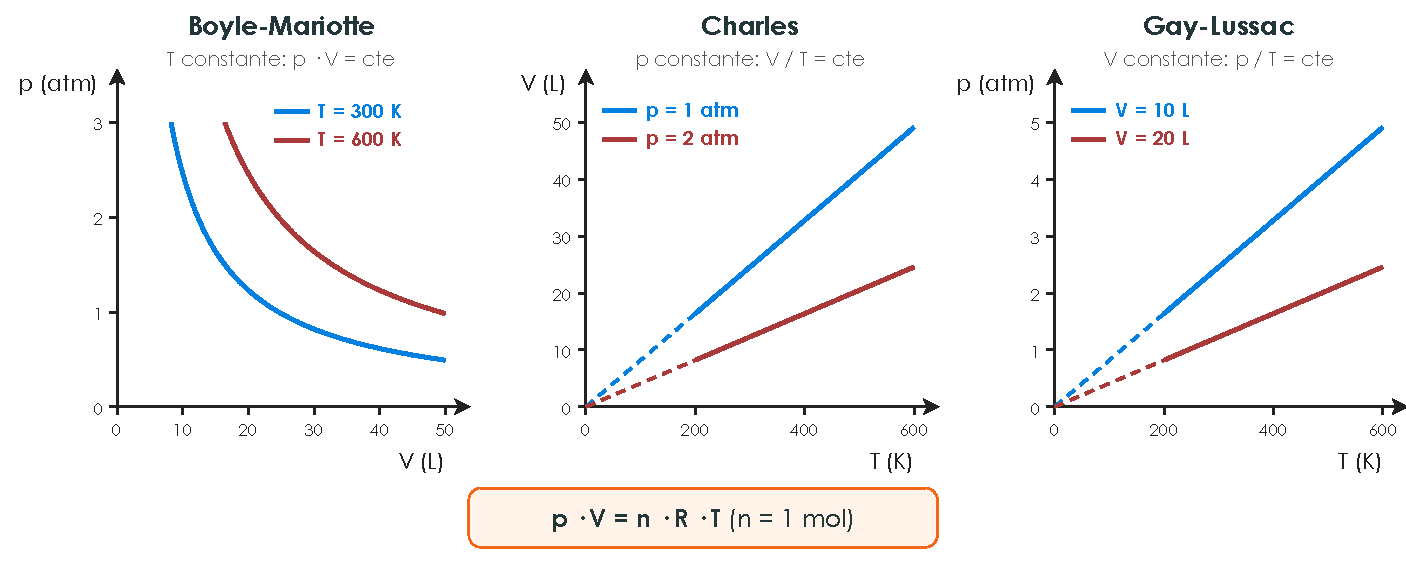
\includegraphics[width=1.0\linewidth]{FigurasSVG/UD0_Conocimientos_Basicos/pdf/UD0_04_leyes_gases.pdf}
    \caption{Leyes de Boyle-Mariotte, Charles y Gay-Lussac (calculadas para \qty{1}{\mol} de gas ideal)}
    \label{fig:leyes-gases}
\end{figure}

Si tomamos el valor  \( R = \ctegases \) debemos tener la presión en atmósferas, la temperatura en Kelvin y el volumen en litros.

\begin{definition}[volumen molar]
    es el volumen ocupado por un mol de un gas ideal que será siempre el mismo en las mismas condiciones de presión y temperatura.
\end{definition}

Llamamos condiciones normales (cn) cuando la presión \( p = \qty{1}{\atmosphere} \) y la temperatura \( T = \qty{0}{\celsius} \longrightarrow T = \qty{273}{\kelvin}\). El volumen ocupado por cualquier gas ideal en estas condiciones siempre es de \( V_{{cn}} = \qty{22.4}{\litre} \). En la última actualización, la IUPAC acepta establecer este volumen molar en condiciones normales como \(V_{cn} \qty{22.7}{\litre} \). Este cambio se debe a que el factor de conversión entre Pascales (\unit{\pascal}) y atmósferas (\unit{\atmosphere}) ha pasado de \( \qty{1}{\atmosphere} = \qty{101325}{\pascal} \) a \( \qty{1}{\atmosphere} = \qty{e5}{\pascal} \).

\subsection{Ley de Dalton}

\begin{ley}[Ley de Dalton]
    La ley de Dalton o también llamada ley de las presiones parciales dice que: en una mezcla de gases, la presión total es la suma de las presiones parciales que ejerce cada gas de manera individual.
    \begin{centeredequation}
        p_T = \sum_{i=m}^{n} p_i \longrightarrow p_T = p_{m} + p_{m+1} + p_{m+1} + ... + p_{n}
    \end{centeredequation}
\end{ley}

Si tenemos una mezcla de \( \ch{CO2} + \ch{CO} + \ch{H2} \) en un recipiente cerrado la presión total de la mezcla será la suma de las presiones de cada compuesto quedando que
\begin{centeredequation*}
    p_T = p_{\ch{CO2}} + p_{\ch{CO}} + p_{\ch{H2}}
\end{centeredequation*}

De esta ley se deduce que la presión de un determinado componente de la mezcla será igual al producto entre la fracción molar de ese componente por la presión total. Si consideramos el compuesto \( i \) en una mezcla tendremos que:
\begin{centeredequation}
    p_i = \chi_i \cdot p_T
\end{centeredequation}


\begin{figure}[H]
    \centering
    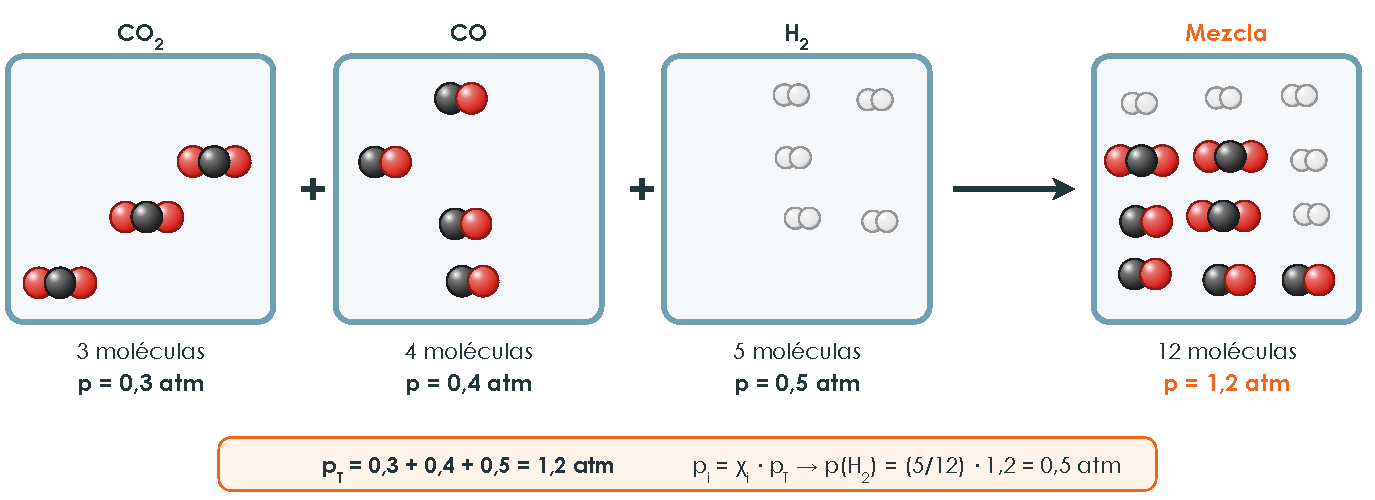
\includegraphics[width=1.0\linewidth]{FigurasSVG/UD0_Conocimientos_Basicos/pdf/UD0_05_ley_dalton.pdf}
    \caption{Ley de Dalton: la presión total es la suma de las presiones parciales}
    \label{fig:ley-dalton}
\end{figure}

\section{Fórmulas}

En los compuestos iónicos, la fórmula indica la proporción en la que se encuentran los iones en el cristal, mientras que para los compuestos covalentes se pueden utilizar varios tipos de fórmulas:
\begin{itemize}
    \item \negsubro{Fórmula empírica:} indica la mínima relación entre átomos de una molécula.
    \item \negsubro{Fórmula molecular:} indica el número real de átomos que forman la molécula.
    \item \textbf{Fórmula estructural:} indica como están enlazados los átomos en la molécula.
\end{itemize}

En los compuestos inorgánicos (excepto los peróxidos), las fórmulas empírica y molecular coinciden, pero no es así en los compuestos orgánicos.

\begin{example}
    Para el agua tendremos que:
    \begin{itemize}
        \item La fórmula empírica es \ch{H2O}.
        \item La fórmula molecular es \ch{H2O}.
    \end{itemize}
    Para el peróxido de hidrógeno tendremos que:
    \begin{itemize}
        \item La fórmula empírica es \ch{HO}.
        \item La fórmula molecular es \ch{H2O2}.
    \end{itemize}
    Para el etano tendremos que:
    \begin{itemize}
        \item La fórmula empírica es \ch{CH3}.
        \item La fórmula molecular es \ch{C2H6}.
    \end{itemize}

\end{example}


\begin{figure}[H]
    \centering
    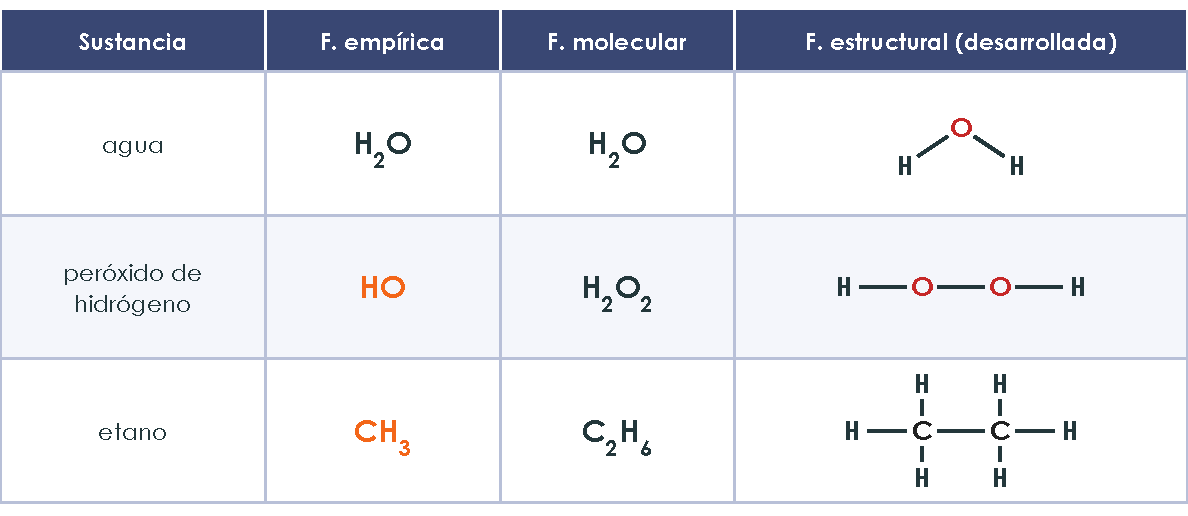
\includegraphics[width=0.8\linewidth]{FigurasSVG/UD0_Conocimientos_Basicos/pdf/UD0_06_tipos_formulas.pdf}
    \caption{Fórmulas empírica, molecular y estructural}
    \label{fig:tipos-formulas}
\end{figure}

\section{Reacciones químicas}

Una reacción química es el proceso mediante el cual, a partir de unas sustancias llamadas reactivos se obtienen otras sustancias distintas llamadas productos.
Las reacciones se representan mediante las llamadas ecuaciones químicas, en las que aparecen las fórmulas de los reactivos y de los productos separados por una flecha, que indica el sentido en el que tiene lugar la reacción. Ahora bien, como en una reacción la masa se conserva (según la ley de conservación de la masa de Lavoisier), permanece constante, ya que, tan solo tiene lugar la reordenación, el reagrupamiento de los átomos, pero el número de átomos de cada elemento es el mismo antes y después de la reacción, para que la ecuación química esté completa, tiene que estar ajustada y para ello se introducen unos coeficientes que indican el número de moléculas (y por tanto, también de moles) de cada sustancia, que intervienen en la reacción.

\begin{centeredequation}
    \ch{N2 + 3 H2 -> 2 NH3}
\end{centeredequation}

En este ejemplo, podemos ver como 1 molécula de \ch{N2} reacciona con 3 moléculas de \ch{H2} para formar 2 moléculas de \ch{NH3}. Podemos decir también que 1 mol de \ch{N2} reacciona con 3 moles de \ch{H2} para formar 2 moles de \ch{NH3}.

\begin{figure}[H]
    \centering
    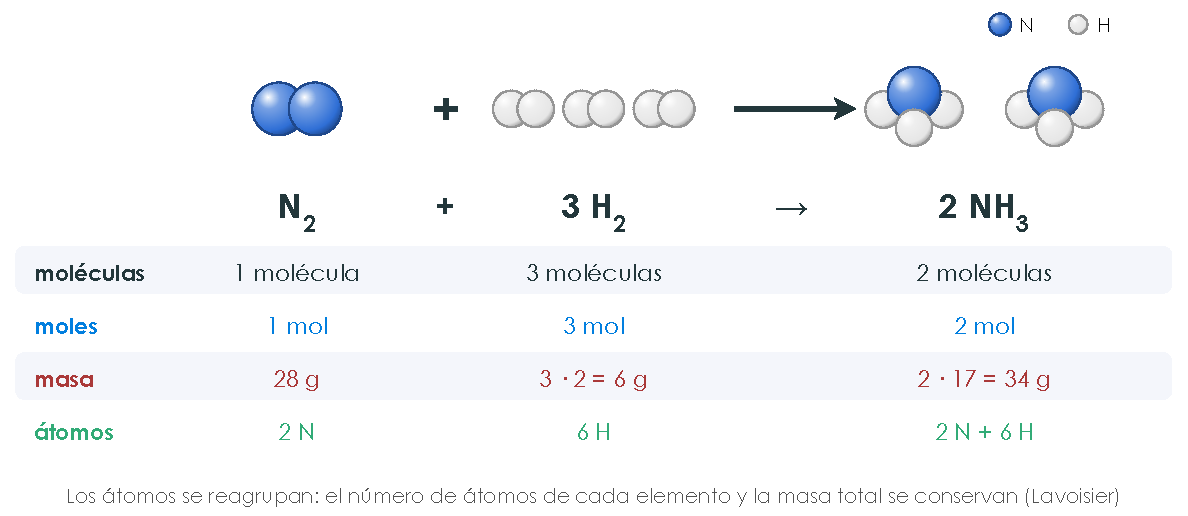
\includegraphics[width=0.8\linewidth]{FigurasSVG/UD0_Conocimientos_Basicos/pdf/UD0_07_reaccion_N2_H2.pdf}
    \caption{Interpretación de la ecuación química \ch{N2 + 3 H2 -> 2 NH3}}
    \label{fig:reaccion-N2-H2}
\end{figure}

\subsection{Cálculos estequiométricos}

La estequiometría es el estudio cuantitativo de las reacciones. Conocida la cantidad de una sustancia, se puede calcular la cantidad de otra sustancia que intervenga en la reacción, valiéndonos de los coeficientes estequiométricos, ya que éstos indican la relación en moles, y en el caso de que todas las sustancias sean gaseosas también indican la relación en volumen (litros, \unit{\cubic\centi\metre},etc.), lo cual se deduce de la hipótesis de Avogadro.

Con la estequiometría, podemos:
\begin{itemize}
    \item Se pueden determinar las cantidades de reactivos y productos, mediante relaciones mol-mol, masa-masa, masa-volumen, volumen-volumen.
    \item En muchas reacciones, las cantidades de los reactivos no están en las proporciones exactas de reacción; en tal caso, las cantidades obtenidas de los productos, están determinadas por el reactivo limitante, esto es, el reactivo que se consume antes.
    \item En la práctica, la mayoría de las veces no se obtiene la cantidad de producto que se deduce de la estequiometría de la reacción, debido a que, no llegan a consumirse totalmente los reactivos y que además de la reacción principal se producen otras reacciones secundarias, lo que hace que el rendimiento de la reacción no sea del 100\%.
    \begin{centeredequation}
        \text{\% de rendimiento} = \dfrac{\text{cantidad del producto obtenido experimentalmente}}{\text{cantidad del producto que se debe obtener de forma teórica}} \times 100
    \end{centeredequation}
    Por ejemplo, un rendimiento del 80\% significa que de cada \qty{100}{\mol} que teóricamente deberían obtenerse, en la práctica tan solo se han obtenido \qty{80}{\mol}.
    \begin{remark}
        Para evitar errores en los cálculos estequiométricos se aconseja siempre pasar todo y trabajar en los cálculos con moles y luego calcular los gramos de cada sustancia según se pida.
    \end{remark}
    \item A veces, el reactivo no es puro o se encuentra en disolución como soluto; en tal caso, hay que determinar la cantidad de reactivo que realmente interviene en la reacción. Si un compuesto tiene una pureza del 70\% (si no se especifica, supondremos que el porcentaje será en masa) quiere decir que de \qty{100}{\g} de ese compuesto, tan solo \qty{70}{\g} son puros.
\end{itemize}

\begin{figure}[H]
    \centering
    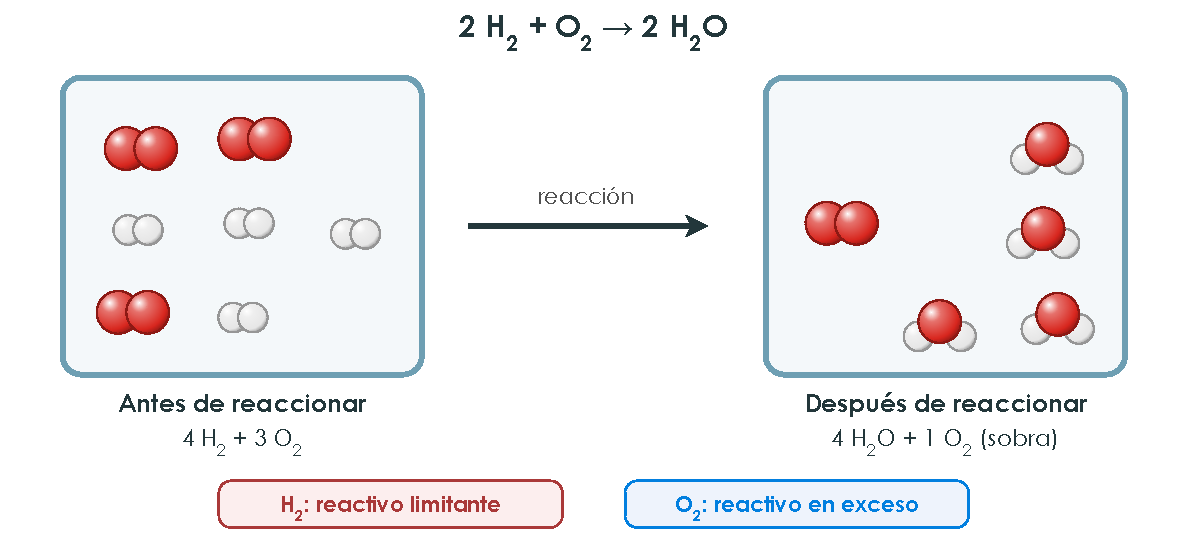
\includegraphics[width=0.75\linewidth]{FigurasSVG/UD0_Conocimientos_Basicos/pdf/UD0_08_reactivo_limitante.pdf}
    \caption{Reactivo limitante y reactivo en exceso}
    \label{fig:reactivo-limitante}
\end{figure}

\begin{figure}[H]
    \centering
    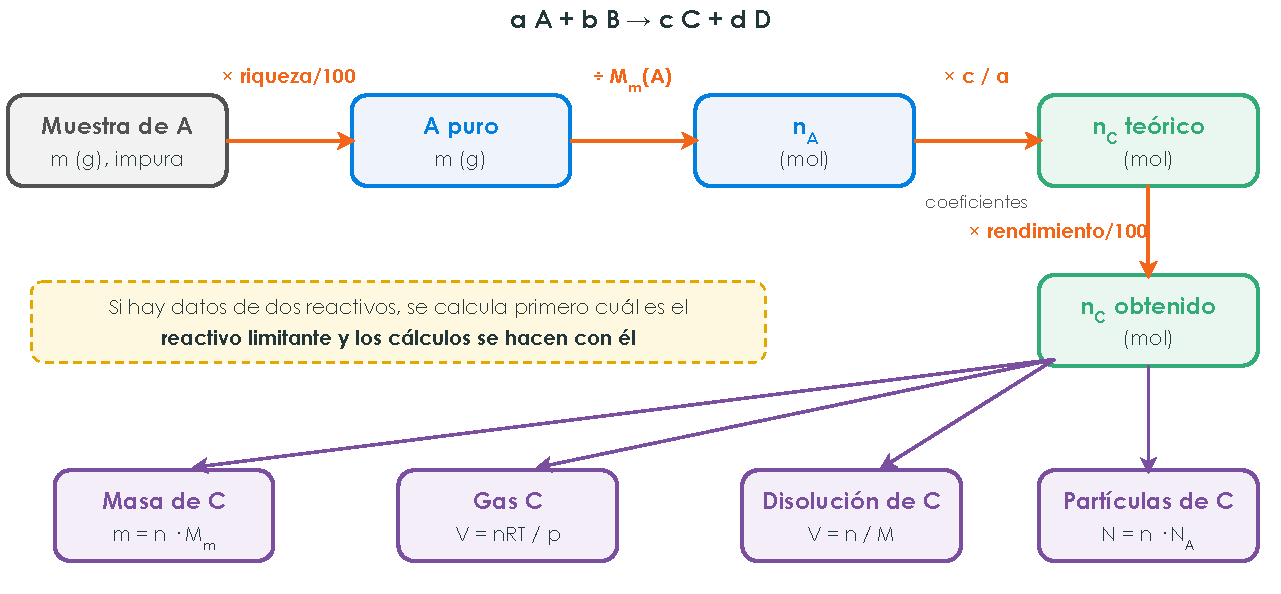
\includegraphics[width=0.9\linewidth]{FigurasSVG/UD0_Conocimientos_Basicos/pdf/UD0_09_ruta_estequiometrica.pdf}
    \caption{Pasos de un cálculo estequiométrico}
    \label{fig:ruta-estequiometrica}
\end{figure}
